\documentclass[twoside]{book}

% Packages required by doxygen
\usepackage{calc}
\usepackage{doxygen}
\usepackage{graphicx}
\usepackage[utf8]{inputenc}
\usepackage{makeidx}
\usepackage{multicol}
\usepackage{multirow}
\usepackage{textcomp}
\usepackage[table]{xcolor}

% Font selection
\usepackage[T1]{fontenc}
\usepackage{mathptmx}
\usepackage[scaled=.90]{helvet}
\usepackage{courier}
\usepackage{amssymb}
\usepackage{sectsty}
\renewcommand{\familydefault}{\sfdefault}
\allsectionsfont{%
  \fontseries{bc}\selectfont%
  \color{darkgray}%
}
\renewcommand{\DoxyLabelFont}{%
  \fontseries{bc}\selectfont%
  \color{darkgray}%
}

% Page & text layout
\usepackage{geometry}
\geometry{%
  a4paper,%
  top=2.5cm,%
  bottom=2.5cm,%
  left=2.5cm,%
  right=2.5cm%
}
\tolerance=750
\hfuzz=15pt
\hbadness=750
\setlength{\emergencystretch}{15pt}
\setlength{\parindent}{0cm}
\setlength{\parskip}{0.2cm}
\makeatletter
\renewcommand{\paragraph}{%
  \@startsection{paragraph}{4}{0ex}{-1.0ex}{1.0ex}{%
    \normalfont\normalsize\bfseries\SS@parafont%
  }%
}
\renewcommand{\subparagraph}{%
  \@startsection{subparagraph}{5}{0ex}{-1.0ex}{1.0ex}{%
    \normalfont\normalsize\bfseries\SS@subparafont%
  }%
}
\makeatother

% Headers & footers
\usepackage{fancyhdr}
\pagestyle{fancyplain}
\fancyhead[LE]{\fancyplain{}{\bfseries\thepage}}
\fancyhead[CE]{\fancyplain{}{}}
\fancyhead[RE]{\fancyplain{}{\bfseries\leftmark}}
\fancyhead[LO]{\fancyplain{}{\bfseries\rightmark}}
\fancyhead[CO]{\fancyplain{}{}}
\fancyhead[RO]{\fancyplain{}{\bfseries\thepage}}
\fancyfoot[LE]{\fancyplain{}{}}
\fancyfoot[CE]{\fancyplain{}{}}
\fancyfoot[RE]{\fancyplain{}{\bfseries\scriptsize Generated on Fri May 31 2019 14\-:28\-:04 for Tool\-D\-A\-Q\-Framework by Doxygen }}
\fancyfoot[LO]{\fancyplain{}{\bfseries\scriptsize Generated on Fri May 31 2019 14\-:28\-:04 for Tool\-D\-A\-Q\-Framework by Doxygen }}
\fancyfoot[CO]{\fancyplain{}{}}
\fancyfoot[RO]{\fancyplain{}{}}
\renewcommand{\footrulewidth}{0.4pt}
\renewcommand{\chaptermark}[1]{%
  \markboth{#1}{}%
}
\renewcommand{\sectionmark}[1]{%
  \markright{\thesection\ #1}%
}

% Indices & bibliography
\usepackage{natbib}
\usepackage[titles]{tocloft}
\setcounter{tocdepth}{3}
\setcounter{secnumdepth}{5}
\makeindex

% Hyperlinks (required, but should be loaded last)
\usepackage{ifpdf}
\ifpdf
  \usepackage[pdftex,pagebackref=true]{hyperref}
\else
  \usepackage[ps2pdf,pagebackref=true]{hyperref}
\fi
\hypersetup{%
  colorlinks=true,%
  linkcolor=blue,%
  citecolor=blue,%
  unicode%
}

% Custom commands
\newcommand{\clearemptydoublepage}{%
  \newpage{\pagestyle{empty}\cleardoublepage}%
}


%===== C O N T E N T S =====

\begin{document}

% Titlepage & ToC
\hypersetup{pageanchor=false}
\pagenumbering{roman}
\begin{titlepage}
\vspace*{7cm}
\begin{center}%
{\Large Tool\-D\-A\-Q\-Framework }\\
\vspace*{1cm}
{\large Generated by Doxygen 1.8.5}\\
\vspace*{0.5cm}
{\small Fri May 31 2019 14:28:04}\\
\end{center}
\end{titlepage}
\clearemptydoublepage
\tableofcontents
\clearemptydoublepage
\pagenumbering{arabic}
\hypersetup{pageanchor=true}

%--- Begin generated contents ---
\chapter{Dummy Tool R\-E\-A\-D\-M\-E}
\label{md_UserTools_DummyTool_README}
\hypertarget{md_UserTools_DummyTool_README}{}
\subsection*{Data}

This Tool Is just a dummy that prints out differnt messges to the consol depending on the debug level.

\subsection*{Configuration}

Describe any configuration variables for \hyperlink{classMyTool}{My\-Tool}.

verbose value \# any int for the value 
\chapter{D\-A\-Q\-Framework}
\label{md_UserTools_README}
\hypertarget{md_UserTools_README}{}
\input{md_UserTools_README}
\chapter{My\-Tool}
\label{md_UserTools_template_README}
\hypertarget{md_UserTools_template_README}{}
\hyperlink{classMyTool}{My\-Tool}

\subsection*{Data}

Describe any data formats \hyperlink{classMyTool}{My\-Tool} creates, destroys, changes, or analyzes. E.\-G.

{\bfseries Raw\-L\-A\-P\-P\-D\-Data} {\ttfamily map$<$\hyperlink{classGeometry}{Geometry}, vector$<$\hyperlink{classWaveform}{Waveform}$<$double$>$$>$$>$}
\begin{DoxyItemize}
\item Takes this data from the {\ttfamily A\-N\-N\-I\-E\-Event} store and finds the number of peaks
\end{DoxyItemize}

\subsection*{Configuration}

Describe any configuration variables for \hyperlink{classMyTool}{My\-Tool}.

``` param1 value1 param2 value2 ``` 
\chapter{R\-E\-A\-D\-M\-E}
\label{md_DataModel_README}
\hypertarget{md_DataModel_README}{}
\#\-Data Model 



Data Model Class can be defined how ever the User requires. A Store is provided which ineficently maps variables to string lkeys via conversion to stringstream and can be used for debuging or other useful vairables.

A T\-Tree map with getter and setter functions is provided and can be uncommented if required. 
\chapter{Hierarchical Index}
\section{Class Hierarchy}
This inheritance list is sorted roughly, but not completely, alphabetically\-:\begin{DoxyCompactList}
\item \contentsline{section}{A\-N\-N\-I\-E\-Geometry}{\pageref{classANNIEGeometry}}{}
\item \contentsline{section}{A\-N\-N\-I\-E\-Reco\-Object\-Table}{\pageref{classANNIERecoObjectTable}}{}
\item \contentsline{section}{Card\-Data}{\pageref{classCardData}}{}
\item \contentsline{section}{Data\-Model}{\pageref{classDataModel}}{}
\item \contentsline{section}{Example\-Root}{\pageref{classExampleRoot}}{}
\item \contentsline{section}{Fo\-M\-Calculator}{\pageref{classFoMCalculator}}{}
\item \contentsline{section}{annie\-:\-:Hefty\-Tree\-Reader}{\pageref{classannie_1_1HeftyTreeReader}}{}
\item \contentsline{section}{I\-F\-Beam\-D\-B\-Interface}{\pageref{classIFBeamDBInterface}}{}
\item \contentsline{section}{L\-A\-P\-P\-D}{\pageref{classLAPPD}}{}
\item \contentsline{section}{L\-A\-P\-P\-Dresponse}{\pageref{classLAPPDresponse}}{}
\item \contentsline{section}{L\-A\-P\-P\-D\-Tree}{\pageref{classLAPPDTree}}{}
\item \contentsline{section}{Minuit\-Optimizer}{\pageref{classMinuitOptimizer}}{}
\item \contentsline{section}{M\-R\-D\-Tree}{\pageref{classMRDTree}}{}
\item \contentsline{section}{N\-C\-V\-Position\-Info}{\pageref{structNCVPositionInfo}}{}
\item \contentsline{section}{Parameters}{\pageref{classParameters}}{}
\item \contentsline{section}{P\-M\-T\-Data}{\pageref{classPMTData}}{}
\item \contentsline{section}{quaternion}{\pageref{structquaternion}}{}
\item \contentsline{section}{annie\-:\-:Raw\-Analyzer}{\pageref{classannie_1_1RawAnalyzer}}{}
\item \contentsline{section}{annie\-:\-:Raw\-Card}{\pageref{classannie_1_1RawCard}}{}
\item \contentsline{section}{annie\-:\-:Raw\-Channel}{\pageref{classannie_1_1RawChannel}}{}
\item \contentsline{section}{annie\-:\-:Raw\-Reader}{\pageref{classannie_1_1RawReader}}{}
\item \contentsline{section}{annie\-:\-:Raw\-Readout}{\pageref{classannie_1_1RawReadout}}{}
\item \contentsline{section}{annie\-:\-:Raw\-Trig\-Data}{\pageref{classannie_1_1RawTrigData}}{}
\item \contentsline{section}{annie\-:\-:Reco\-Pulse}{\pageref{classannie_1_1RecoPulse}}{}
\item \contentsline{section}{annie\-:\-:Reco\-Readout}{\pageref{classannie_1_1RecoReadout}}{}
\item Serialisable\-Object\begin{DoxyCompactList}
\item \contentsline{section}{Beam\-Data\-Point}{\pageref{structBeamDataPoint}}{}
\item \contentsline{section}{Beam\-Status}{\pageref{classBeamStatus}}{}
\item \contentsline{section}{Beam\-Status\-Class}{\pageref{classBeamStatusClass}}{}
\item \contentsline{section}{Channel}{\pageref{classChannel}}{}
\item \contentsline{section}{Channel\-Key}{\pageref{classChannelKey}}{}
\item \contentsline{section}{Detector}{\pageref{classDetector}}{}
\item \contentsline{section}{Direction}{\pageref{classDirection}}{}
\item \contentsline{section}{Geometry}{\pageref{classGeometry}}{}
\item \contentsline{section}{Hefty\-Info}{\pageref{classHeftyInfo}}{}
\item \contentsline{section}{Hit}{\pageref{classHit}}{}
\begin{DoxyCompactList}
\item \contentsline{section}{A\-D\-C\-Pulse}{\pageref{classADCPulse}}{}
\item \contentsline{section}{L\-A\-P\-P\-D\-Hit}{\pageref{classLAPPDHit}}{}
\begin{DoxyCompactList}
\item \contentsline{section}{M\-C\-L\-A\-P\-P\-D\-Hit}{\pageref{classMCLAPPDHit}}{}
\end{DoxyCompactList}
\item \contentsline{section}{L\-A\-P\-P\-D\-Pulse}{\pageref{classLAPPDPulse}}{}
\item \contentsline{section}{M\-C\-Hit}{\pageref{classMCHit}}{}
\end{DoxyCompactList}
\item \contentsline{section}{M\-R\-D\-Out}{\pageref{classMRDOut}}{}
\item \contentsline{section}{Particle}{\pageref{classParticle}}{}
\begin{DoxyCompactList}
\item \contentsline{section}{M\-C\-Particle}{\pageref{classMCParticle}}{}
\end{DoxyCompactList}
\item \contentsline{section}{Position}{\pageref{classPosition}}{}
\item \contentsline{section}{Reco\-Cluster}{\pageref{classRecoCluster}}{}
\item \contentsline{section}{Reco\-Cluster\-Digit}{\pageref{classRecoClusterDigit}}{}
\item \contentsline{section}{Reco\-Digit}{\pageref{classRecoDigit}}{}
\item \contentsline{section}{Reco\-Ring}{\pageref{classRecoRing}}{}
\item \contentsline{section}{Reco\-Vertex}{\pageref{classRecoVertex}}{}
\item \contentsline{section}{Time\-Class}{\pageref{classTimeClass}}{}
\item \contentsline{section}{Trigger\-Class}{\pageref{classTriggerClass}}{}
\item \contentsline{section}{Waveform$<$ T $>$}{\pageref{classWaveform}}{}
\begin{DoxyCompactList}
\item \contentsline{section}{Calibrated\-A\-D\-C\-Waveform$<$ T $>$}{\pageref{classCalibratedADCWaveform}}{}
\end{DoxyCompactList}
\end{DoxyCompactList}
\item \contentsline{section}{T\-Banded\-L\-E}{\pageref{classTBandedLE}}{}
\item T\-Named\begin{DoxyCompactList}
\item \contentsline{section}{T\-One\-Pad\-Display}{\pageref{classTOnePadDisplay}}{}
\item \contentsline{section}{T\-Spline\-Fit}{\pageref{classTSplineFit}}{}
\end{DoxyCompactList}
\item Tool\begin{DoxyCompactList}
\item \contentsline{section}{A\-D\-C\-Calibrator}{\pageref{classADCCalibrator}}{}
\item \contentsline{section}{A\-D\-C\-Hit\-Finder}{\pageref{classADCHitFinder}}{}
\item \contentsline{section}{Beam\-Checker}{\pageref{classBeamChecker}}{}
\item \contentsline{section}{Beam\-Fetcher}{\pageref{classBeamFetcher}}{}
\item \contentsline{section}{Beam\-Time\-Ana}{\pageref{classBeamTimeAna}}{}
\item \contentsline{section}{Beam\-Time\-Tree\-Maker}{\pageref{classBeamTimeTreeMaker}}{}
\item \contentsline{section}{Beam\-Time\-Tree\-Reader}{\pageref{classBeamTimeTreeReader}}{}
\item \contentsline{section}{Check\-Detector\-Counts}{\pageref{classCheckDetectorCounts}}{}
\item \contentsline{section}{Digit\-Builder}{\pageref{classDigitBuilder}}{}
\item \contentsline{section}{Digit\-Builder\-Do\-E}{\pageref{classDigitBuilderDoE}}{}
\item \contentsline{section}{Digit\-Builder\-R\-O\-O\-T}{\pageref{classDigitBuilderROOT}}{}
\item \contentsline{section}{Dummy\-Tool}{\pageref{classDummyTool}}{}
\item \contentsline{section}{Event\-Display}{\pageref{classEventDisplay}}{}
\item \contentsline{section}{Event\-Selector}{\pageref{classEventSelector}}{}
\item \contentsline{section}{Event\-Selector\-Do\-E}{\pageref{classEventSelectorDoE}}{}
\item \contentsline{section}{Example\-Generate\-Data}{\pageref{classExampleGenerateData}}{}
\item \contentsline{section}{Example\-Load\-Root}{\pageref{classExampleLoadRoot}}{}
\item \contentsline{section}{Exampleload\-Store}{\pageref{classExampleloadStore}}{}
\item \contentsline{section}{Example\-Over\-Tool}{\pageref{classExampleOverTool}}{}
\item \contentsline{section}{Example\-Print\-Data}{\pageref{classExamplePrintData}}{}
\item \contentsline{section}{Example\-Save\-Root}{\pageref{classExampleSaveRoot}}{}
\item \contentsline{section}{Example\-Save\-Store}{\pageref{classExampleSaveStore}}{}
\item \contentsline{section}{Find\-Mrd\-Tracks}{\pageref{classFindMrdTracks}}{}
\item \contentsline{section}{Find\-Track\-Length\-In\-Water}{\pageref{classFindTrackLengthInWater}}{}
\item \contentsline{section}{Generate\-Hits}{\pageref{classGenerateHits}}{}
\item \contentsline{section}{Histograms\-Root\-L\-A\-P\-P\-D\-Data}{\pageref{classHistogramsRootLAPPDData}}{}
\item \contentsline{section}{Hit\-Cleaner}{\pageref{classHitCleaner}}{}
\item \contentsline{section}{Hit\-Residuals}{\pageref{classHitResiduals}}{}
\item \contentsline{section}{L\-A\-P\-P\-D\-Analysis}{\pageref{classLAPPDAnalysis}}{}
\item \contentsline{section}{L\-A\-P\-P\-D\-Baseline\-Subtract}{\pageref{classLAPPDBaselineSubtract}}{}
\item \contentsline{section}{L\-A\-P\-P\-Dcfd}{\pageref{classLAPPDcfd}}{}
\item \contentsline{section}{L\-A\-P\-P\-D\-Filter}{\pageref{classLAPPDFilter}}{}
\item \contentsline{section}{L\-A\-P\-P\-D\-Find\-Peak}{\pageref{classLAPPDFindPeak}}{}
\item \contentsline{section}{L\-A\-P\-P\-D\-Integrate\-Pulse}{\pageref{classLAPPDIntegratePulse}}{}
\item \contentsline{section}{L\-A\-P\-P\-Dlasertest\-Hit\-Finder}{\pageref{classLAPPDlasertestHitFinder}}{}
\item \contentsline{section}{L\-A\-P\-P\-D\-Parse\-A\-C\-C}{\pageref{classLAPPDParseACC}}{}
\item \contentsline{section}{L\-A\-P\-P\-D\-Parse\-Scope}{\pageref{classLAPPDParseScope}}{}
\item \contentsline{section}{L\-A\-P\-P\-D\-Save\-R\-O\-O\-T}{\pageref{classLAPPDSaveROOT}}{}
\item \contentsline{section}{L\-A\-P\-P\-D\-Sim}{\pageref{classLAPPDSim}}{}
\item \contentsline{section}{Likelihood\-Fitter\-Check}{\pageref{classLikelihoodFitterCheck}}{}
\item \contentsline{section}{Load\-A\-N\-N\-I\-E\-Event}{\pageref{classLoadANNIEEvent}}{}
\item \contentsline{section}{Load\-C\-C\-Data}{\pageref{classLoadCCData}}{}
\item \contentsline{section}{Load\-Geometry}{\pageref{classLoadGeometry}}{}
\item \contentsline{section}{Load\-W\-C\-Sim}{\pageref{classLoadWCSim}}{}
\item \contentsline{section}{Load\-W\-C\-Sim\-L\-A\-P\-P\-D}{\pageref{classLoadWCSimLAPPD}}{}
\item \contentsline{section}{M\-C\-Particle\-Properties}{\pageref{classMCParticleProperties}}{}
\item \contentsline{section}{M\-C\-Reco\-Event\-Loader}{\pageref{classMCRecoEventLoader}}{}
\item \contentsline{section}{Monitor\-M\-R\-D\-Live}{\pageref{classMonitorMRDLive}}{}
\item \contentsline{section}{Monitor\-M\-R\-D\-Time}{\pageref{classMonitorMRDTime}}{}
\item \contentsline{section}{Monitor\-Receive}{\pageref{classMonitorReceive}}{}
\item \contentsline{section}{Monitor\-Sim\-Receive}{\pageref{classMonitorSimReceive}}{}
\item \contentsline{section}{Mrd\-Discriminator\-Scan}{\pageref{classMrdDiscriminatorScan}}{}
\item \contentsline{section}{Mrd\-Distributions}{\pageref{classMrdDistributions}}{}
\item \contentsline{section}{Mrd\-Efficiency}{\pageref{classMrdEfficiency}}{}
\item \contentsline{section}{Mrd\-Paddle\-Plot}{\pageref{classMrdPaddlePlot}}{}
\item \contentsline{section}{M\-R\-D\-Pulse\-Finder}{\pageref{classMRDPulseFinder}}{}
\item \contentsline{section}{My\-Tool}{\pageref{classMyTool}}{}
\item \contentsline{section}{Neutron\-Study\-P\-M\-C\-S}{\pageref{classNeutronStudyPMCS}}{}
\item \contentsline{section}{Neutron\-Study\-Read\-Sandbox}{\pageref{classNeutronStudyReadSandbox}}{}
\item \contentsline{section}{Neutron\-Study\-Write\-Tree}{\pageref{classNeutronStudyWriteTree}}{}
\item \contentsline{section}{Phase\-I\-I\-Tree\-Maker}{\pageref{classPhaseIITreeMaker}}{}
\item \contentsline{section}{Phase\-I\-Tree\-Maker}{\pageref{classPhaseITreeMaker}}{}
\item \contentsline{section}{Plot\-L\-A\-P\-P\-D\-Times\-From\-Store}{\pageref{classPlotLAPPDTimesFromStore}}{}
\item \contentsline{section}{Print\-A\-N\-N\-I\-E\-Event}{\pageref{classPrintANNIEEvent}}{}
\item \contentsline{section}{Pulse\-Simulation}{\pageref{classPulseSimulation}}{}
\item \contentsline{section}{Python\-Script}{\pageref{classPythonScript}}{}
\item \contentsline{section}{Raw\-Loader}{\pageref{classRawLoader}}{}
\item \contentsline{section}{Raw\-Load\-To\-Root}{\pageref{classRawLoadToRoot}}{}
\item \contentsline{section}{Save\-A\-N\-N\-I\-E\-Event}{\pageref{classSaveANNIEEvent}}{}
\item \contentsline{section}{Save\-Reco\-Event}{\pageref{classSaveRecoEvent}}{}
\item \contentsline{section}{Tank\-Calibration\-Diffuser}{\pageref{classTankCalibrationDiffuser}}{}
\item \contentsline{section}{Total\-Light\-Map}{\pageref{classTotalLightMap}}{}
\item \contentsline{section}{Vertex\-Geometry\-Check}{\pageref{classVertexGeometryCheck}}{}
\item \contentsline{section}{Vtx\-Extended\-Vertex\-Finder}{\pageref{classVtxExtendedVertexFinder}}{}
\item \contentsline{section}{Vtx\-Point\-Direction\-Finder}{\pageref{classVtxPointDirectionFinder}}{}
\item \contentsline{section}{Vtx\-Point\-Position\-Finder}{\pageref{classVtxPointPositionFinder}}{}
\item \contentsline{section}{Vtx\-Point\-Vertex\-Finder}{\pageref{classVtxPointVertexFinder}}{}
\item \contentsline{section}{Vtx\-Seed\-Generator}{\pageref{classVtxSeedGenerator}}{}
\item \contentsline{section}{W\-C\-Sim\-Demo}{\pageref{classWCSimDemo}}{}
\end{DoxyCompactList}
\item \contentsline{section}{T\-Poly3}{\pageref{classTPoly3}}{}
\item \contentsline{section}{T\-Zig\-Zag}{\pageref{classTZigZag}}{}
\item \contentsline{section}{Vertex\-Geometry}{\pageref{classVertexGeometry}}{}
\item \contentsline{section}{Water\-Model\-:\-:water\-M}{\pageref{structWaterModel_1_1waterM}}{}
\item \contentsline{section}{Water\-Model}{\pageref{classWaterModel}}{}
\item \contentsline{section}{wcsim\-T}{\pageref{classwcsimT}}{}
\end{DoxyCompactList}

\chapter{Class Index}
\section{Class List}
Here are the classes, structs, unions and interfaces with brief descriptions\-:\begin{DoxyCompactList}
\item\contentsline{section}{\hyperlink{classADCCalibrator}{A\-D\-C\-Calibrator} }{\pageref{classADCCalibrator}}{}
\item\contentsline{section}{\hyperlink{classADCHitFinder}{A\-D\-C\-Hit\-Finder} }{\pageref{classADCHitFinder}}{}
\item\contentsline{section}{\hyperlink{classADCPulse}{A\-D\-C\-Pulse} }{\pageref{classADCPulse}}{}
\item\contentsline{section}{\hyperlink{classANNIEGeometry}{A\-N\-N\-I\-E\-Geometry} }{\pageref{classANNIEGeometry}}{}
\item\contentsline{section}{\hyperlink{classANNIERecoObjectTable}{A\-N\-N\-I\-E\-Reco\-Object\-Table} }{\pageref{classANNIERecoObjectTable}}{}
\item\contentsline{section}{\hyperlink{classBeamChecker}{Beam\-Checker} }{\pageref{classBeamChecker}}{}
\item\contentsline{section}{\hyperlink{structBeamDataPoint}{Beam\-Data\-Point} \\*Container to hold values from Intensity Frontier beam database queries, together with their associated units }{\pageref{structBeamDataPoint}}{}
\item\contentsline{section}{\hyperlink{classBeamFetcher}{Beam\-Fetcher} }{\pageref{classBeamFetcher}}{}
\item\contentsline{section}{\hyperlink{classBeamStatus}{Beam\-Status} }{\pageref{classBeamStatus}}{}
\item\contentsline{section}{\hyperlink{classBeamStatusClass}{Beam\-Status\-Class} }{\pageref{classBeamStatusClass}}{}
\item\contentsline{section}{\hyperlink{classBeamTimeAna}{Beam\-Time\-Ana} }{\pageref{classBeamTimeAna}}{}
\item\contentsline{section}{\hyperlink{classBeamTimeTreeMaker}{Beam\-Time\-Tree\-Maker} }{\pageref{classBeamTimeTreeMaker}}{}
\item\contentsline{section}{\hyperlink{classBeamTimeTreeReader}{Beam\-Time\-Tree\-Reader} }{\pageref{classBeamTimeTreeReader}}{}
\item\contentsline{section}{\hyperlink{classCalibratedADCWaveform}{Calibrated\-A\-D\-C\-Waveform$<$ T $>$} }{\pageref{classCalibratedADCWaveform}}{}
\item\contentsline{section}{\hyperlink{classCardData}{Card\-Data} }{\pageref{classCardData}}{}
\item\contentsline{section}{\hyperlink{classChannel}{Channel} }{\pageref{classChannel}}{}
\item\contentsline{section}{\hyperlink{classChannelKey}{Channel\-Key} }{\pageref{classChannelKey}}{}
\item\contentsline{section}{\hyperlink{classCheckDetectorCounts}{Check\-Detector\-Counts} }{\pageref{classCheckDetectorCounts}}{}
\item\contentsline{section}{\hyperlink{classDataModel}{Data\-Model} }{\pageref{classDataModel}}{}
\item\contentsline{section}{\hyperlink{classDetector}{Detector} }{\pageref{classDetector}}{}
\item\contentsline{section}{\hyperlink{classDigitBuilder}{Digit\-Builder} }{\pageref{classDigitBuilder}}{}
\item\contentsline{section}{\hyperlink{classDigitBuilderDoE}{Digit\-Builder\-Do\-E} }{\pageref{classDigitBuilderDoE}}{}
\item\contentsline{section}{\hyperlink{classDigitBuilderROOT}{Digit\-Builder\-R\-O\-O\-T} }{\pageref{classDigitBuilderROOT}}{}
\item\contentsline{section}{\hyperlink{classDirection}{Direction} }{\pageref{classDirection}}{}
\item\contentsline{section}{\hyperlink{classDummyTool}{Dummy\-Tool} }{\pageref{classDummyTool}}{}
\item\contentsline{section}{\hyperlink{classEventDisplay}{Event\-Display} }{\pageref{classEventDisplay}}{}
\item\contentsline{section}{\hyperlink{classEventSelector}{Event\-Selector} }{\pageref{classEventSelector}}{}
\item\contentsline{section}{\hyperlink{classEventSelectorDoE}{Event\-Selector\-Do\-E} }{\pageref{classEventSelectorDoE}}{}
\item\contentsline{section}{\hyperlink{classExampleGenerateData}{Example\-Generate\-Data} }{\pageref{classExampleGenerateData}}{}
\item\contentsline{section}{\hyperlink{classExampleLoadRoot}{Example\-Load\-Root} }{\pageref{classExampleLoadRoot}}{}
\item\contentsline{section}{\hyperlink{classExampleloadStore}{Exampleload\-Store} }{\pageref{classExampleloadStore}}{}
\item\contentsline{section}{\hyperlink{classExampleOverTool}{Example\-Over\-Tool} }{\pageref{classExampleOverTool}}{}
\item\contentsline{section}{\hyperlink{classExamplePrintData}{Example\-Print\-Data} }{\pageref{classExamplePrintData}}{}
\item\contentsline{section}{\hyperlink{classExampleRoot}{Example\-Root} }{\pageref{classExampleRoot}}{}
\item\contentsline{section}{\hyperlink{classExampleSaveRoot}{Example\-Save\-Root} }{\pageref{classExampleSaveRoot}}{}
\item\contentsline{section}{\hyperlink{classExampleSaveStore}{Example\-Save\-Store} }{\pageref{classExampleSaveStore}}{}
\item\contentsline{section}{\hyperlink{classFindMrdTracks}{Find\-Mrd\-Tracks} }{\pageref{classFindMrdTracks}}{}
\item\contentsline{section}{\hyperlink{classFindTrackLengthInWater}{Find\-Track\-Length\-In\-Water} }{\pageref{classFindTrackLengthInWater}}{}
\item\contentsline{section}{\hyperlink{classFoMCalculator}{Fo\-M\-Calculator} }{\pageref{classFoMCalculator}}{}
\item\contentsline{section}{\hyperlink{classGenerateHits}{Generate\-Hits} }{\pageref{classGenerateHits}}{}
\item\contentsline{section}{\hyperlink{classGeometry}{Geometry} }{\pageref{classGeometry}}{}
\item\contentsline{section}{\hyperlink{classHeftyInfo}{Hefty\-Info} }{\pageref{classHeftyInfo}}{}
\item\contentsline{section}{\hyperlink{classannie_1_1HeftyTreeReader}{annie\-::\-Hefty\-Tree\-Reader} }{\pageref{classannie_1_1HeftyTreeReader}}{}
\item\contentsline{section}{\hyperlink{classHistogramsRootLAPPDData}{Histograms\-Root\-L\-A\-P\-P\-D\-Data} }{\pageref{classHistogramsRootLAPPDData}}{}
\item\contentsline{section}{\hyperlink{classHit}{Hit} }{\pageref{classHit}}{}
\item\contentsline{section}{\hyperlink{classHitCleaner}{Hit\-Cleaner} }{\pageref{classHitCleaner}}{}
\item\contentsline{section}{\hyperlink{classHitResiduals}{Hit\-Residuals} }{\pageref{classHitResiduals}}{}
\item\contentsline{section}{\hyperlink{classIFBeamDBInterface}{I\-F\-Beam\-D\-B\-Interface} \\*Singleton used to interact with the Intensity Frontier beam database at Fermilab }{\pageref{classIFBeamDBInterface}}{}
\item\contentsline{section}{\hyperlink{classLAPPD}{L\-A\-P\-P\-D} }{\pageref{classLAPPD}}{}
\item\contentsline{section}{\hyperlink{classLAPPDAnalysis}{L\-A\-P\-P\-D\-Analysis} }{\pageref{classLAPPDAnalysis}}{}
\item\contentsline{section}{\hyperlink{classLAPPDBaselineSubtract}{L\-A\-P\-P\-D\-Baseline\-Subtract} }{\pageref{classLAPPDBaselineSubtract}}{}
\item\contentsline{section}{\hyperlink{classLAPPDcfd}{L\-A\-P\-P\-Dcfd} }{\pageref{classLAPPDcfd}}{}
\item\contentsline{section}{\hyperlink{classLAPPDFilter}{L\-A\-P\-P\-D\-Filter} }{\pageref{classLAPPDFilter}}{}
\item\contentsline{section}{\hyperlink{classLAPPDFindPeak}{L\-A\-P\-P\-D\-Find\-Peak} }{\pageref{classLAPPDFindPeak}}{}
\item\contentsline{section}{\hyperlink{classLAPPDHit}{L\-A\-P\-P\-D\-Hit} }{\pageref{classLAPPDHit}}{}
\item\contentsline{section}{\hyperlink{classLAPPDIntegratePulse}{L\-A\-P\-P\-D\-Integrate\-Pulse} }{\pageref{classLAPPDIntegratePulse}}{}
\item\contentsline{section}{\hyperlink{classLAPPDlasertestHitFinder}{L\-A\-P\-P\-Dlasertest\-Hit\-Finder} }{\pageref{classLAPPDlasertestHitFinder}}{}
\item\contentsline{section}{\hyperlink{classLAPPDParseACC}{L\-A\-P\-P\-D\-Parse\-A\-C\-C} }{\pageref{classLAPPDParseACC}}{}
\item\contentsline{section}{\hyperlink{classLAPPDParseScope}{L\-A\-P\-P\-D\-Parse\-Scope} }{\pageref{classLAPPDParseScope}}{}
\item\contentsline{section}{\hyperlink{classLAPPDPulse}{L\-A\-P\-P\-D\-Pulse} }{\pageref{classLAPPDPulse}}{}
\item\contentsline{section}{\hyperlink{classLAPPDresponse}{L\-A\-P\-P\-Dresponse} }{\pageref{classLAPPDresponse}}{}
\item\contentsline{section}{\hyperlink{classLAPPDSaveROOT}{L\-A\-P\-P\-D\-Save\-R\-O\-O\-T} }{\pageref{classLAPPDSaveROOT}}{}
\item\contentsline{section}{\hyperlink{classLAPPDSim}{L\-A\-P\-P\-D\-Sim} }{\pageref{classLAPPDSim}}{}
\item\contentsline{section}{\hyperlink{classLAPPDTree}{L\-A\-P\-P\-D\-Tree} }{\pageref{classLAPPDTree}}{}
\item\contentsline{section}{\hyperlink{classLikelihoodFitterCheck}{Likelihood\-Fitter\-Check} }{\pageref{classLikelihoodFitterCheck}}{}
\item\contentsline{section}{\hyperlink{classLoadANNIEEvent}{Load\-A\-N\-N\-I\-E\-Event} }{\pageref{classLoadANNIEEvent}}{}
\item\contentsline{section}{\hyperlink{classLoadCCData}{Load\-C\-C\-Data} }{\pageref{classLoadCCData}}{}
\item\contentsline{section}{\hyperlink{classLoadGeometry}{Load\-Geometry} }{\pageref{classLoadGeometry}}{}
\item\contentsline{section}{\hyperlink{classLoadWCSim}{Load\-W\-C\-Sim} }{\pageref{classLoadWCSim}}{}
\item\contentsline{section}{\hyperlink{classLoadWCSimLAPPD}{Load\-W\-C\-Sim\-L\-A\-P\-P\-D} }{\pageref{classLoadWCSimLAPPD}}{}
\item\contentsline{section}{\hyperlink{classMCHit}{M\-C\-Hit} }{\pageref{classMCHit}}{}
\item\contentsline{section}{\hyperlink{classMCLAPPDHit}{M\-C\-L\-A\-P\-P\-D\-Hit} }{\pageref{classMCLAPPDHit}}{}
\item\contentsline{section}{\hyperlink{classMCParticle}{M\-C\-Particle} }{\pageref{classMCParticle}}{}
\item\contentsline{section}{\hyperlink{classMCParticleProperties}{M\-C\-Particle\-Properties} }{\pageref{classMCParticleProperties}}{}
\item\contentsline{section}{\hyperlink{classMCRecoEventLoader}{M\-C\-Reco\-Event\-Loader} }{\pageref{classMCRecoEventLoader}}{}
\item\contentsline{section}{\hyperlink{classMinuitOptimizer}{Minuit\-Optimizer} }{\pageref{classMinuitOptimizer}}{}
\item\contentsline{section}{\hyperlink{classMonitorMRDLive}{Monitor\-M\-R\-D\-Live} }{\pageref{classMonitorMRDLive}}{}
\item\contentsline{section}{\hyperlink{classMonitorMRDTime}{Monitor\-M\-R\-D\-Time} }{\pageref{classMonitorMRDTime}}{}
\item\contentsline{section}{\hyperlink{classMonitorReceive}{Monitor\-Receive} }{\pageref{classMonitorReceive}}{}
\item\contentsline{section}{\hyperlink{classMonitorSimReceive}{Monitor\-Sim\-Receive} }{\pageref{classMonitorSimReceive}}{}
\item\contentsline{section}{\hyperlink{classMrdDiscriminatorScan}{Mrd\-Discriminator\-Scan} }{\pageref{classMrdDiscriminatorScan}}{}
\item\contentsline{section}{\hyperlink{classMrdDistributions}{Mrd\-Distributions} }{\pageref{classMrdDistributions}}{}
\item\contentsline{section}{\hyperlink{classMrdEfficiency}{Mrd\-Efficiency} }{\pageref{classMrdEfficiency}}{}
\item\contentsline{section}{\hyperlink{classMRDOut}{M\-R\-D\-Out} }{\pageref{classMRDOut}}{}
\item\contentsline{section}{\hyperlink{classMrdPaddlePlot}{Mrd\-Paddle\-Plot} }{\pageref{classMrdPaddlePlot}}{}
\item\contentsline{section}{\hyperlink{classMRDPulseFinder}{M\-R\-D\-Pulse\-Finder} }{\pageref{classMRDPulseFinder}}{}
\item\contentsline{section}{\hyperlink{classMRDTree}{M\-R\-D\-Tree} }{\pageref{classMRDTree}}{}
\item\contentsline{section}{\hyperlink{classMyTool}{My\-Tool} }{\pageref{classMyTool}}{}
\item\contentsline{section}{\hyperlink{structNCVPositionInfo}{N\-C\-V\-Position\-Info} }{\pageref{structNCVPositionInfo}}{}
\item\contentsline{section}{\hyperlink{classNeutronStudyPMCS}{Neutron\-Study\-P\-M\-C\-S} }{\pageref{classNeutronStudyPMCS}}{}
\item\contentsline{section}{\hyperlink{classNeutronStudyReadSandbox}{Neutron\-Study\-Read\-Sandbox} }{\pageref{classNeutronStudyReadSandbox}}{}
\item\contentsline{section}{\hyperlink{classNeutronStudyWriteTree}{Neutron\-Study\-Write\-Tree} }{\pageref{classNeutronStudyWriteTree}}{}
\item\contentsline{section}{\hyperlink{classParameters}{Parameters} }{\pageref{classParameters}}{}
\item\contentsline{section}{\hyperlink{classParticle}{Particle} }{\pageref{classParticle}}{}
\item\contentsline{section}{\hyperlink{classPhaseIITreeMaker}{Phase\-I\-I\-Tree\-Maker} }{\pageref{classPhaseIITreeMaker}}{}
\item\contentsline{section}{\hyperlink{classPhaseITreeMaker}{Phase\-I\-Tree\-Maker} }{\pageref{classPhaseITreeMaker}}{}
\item\contentsline{section}{\hyperlink{classPlotLAPPDTimesFromStore}{Plot\-L\-A\-P\-P\-D\-Times\-From\-Store} }{\pageref{classPlotLAPPDTimesFromStore}}{}
\item\contentsline{section}{\hyperlink{classPMTData}{P\-M\-T\-Data} }{\pageref{classPMTData}}{}
\item\contentsline{section}{\hyperlink{classPosition}{Position} }{\pageref{classPosition}}{}
\item\contentsline{section}{\hyperlink{classPrintANNIEEvent}{Print\-A\-N\-N\-I\-E\-Event} }{\pageref{classPrintANNIEEvent}}{}
\item\contentsline{section}{\hyperlink{classPulseSimulation}{Pulse\-Simulation} }{\pageref{classPulseSimulation}}{}
\item\contentsline{section}{\hyperlink{classPythonScript}{Python\-Script} }{\pageref{classPythonScript}}{}
\item\contentsline{section}{\hyperlink{structquaternion}{quaternion} }{\pageref{structquaternion}}{}
\item\contentsline{section}{\hyperlink{classannie_1_1RawAnalyzer}{annie\-::\-Raw\-Analyzer} \\*Singleton analyzer class for reconstructing A\-N\-N\-I\-E events from the raw data }{\pageref{classannie_1_1RawAnalyzer}}{}
\item\contentsline{section}{\hyperlink{classannie_1_1RawCard}{annie\-::\-Raw\-Card} }{\pageref{classannie_1_1RawCard}}{}
\item\contentsline{section}{\hyperlink{classannie_1_1RawChannel}{annie\-::\-Raw\-Channel} }{\pageref{classannie_1_1RawChannel}}{}
\item\contentsline{section}{\hyperlink{classRawLoader}{Raw\-Loader} }{\pageref{classRawLoader}}{}
\item\contentsline{section}{\hyperlink{classRawLoadToRoot}{Raw\-Load\-To\-Root} }{\pageref{classRawLoadToRoot}}{}
\item\contentsline{section}{\hyperlink{classannie_1_1RawReader}{annie\-::\-Raw\-Reader} }{\pageref{classannie_1_1RawReader}}{}
\item\contentsline{section}{\hyperlink{classannie_1_1RawReadout}{annie\-::\-Raw\-Readout} }{\pageref{classannie_1_1RawReadout}}{}
\item\contentsline{section}{\hyperlink{classannie_1_1RawTrigData}{annie\-::\-Raw\-Trig\-Data} }{\pageref{classannie_1_1RawTrigData}}{}
\item\contentsline{section}{\hyperlink{classRecoCluster}{Reco\-Cluster} }{\pageref{classRecoCluster}}{}
\item\contentsline{section}{\hyperlink{classRecoClusterDigit}{Reco\-Cluster\-Digit} }{\pageref{classRecoClusterDigit}}{}
\item\contentsline{section}{\hyperlink{classRecoDigit}{Reco\-Digit} }{\pageref{classRecoDigit}}{}
\item\contentsline{section}{\hyperlink{classannie_1_1RecoPulse}{annie\-::\-Reco\-Pulse} }{\pageref{classannie_1_1RecoPulse}}{}
\item\contentsline{section}{\hyperlink{classannie_1_1RecoReadout}{annie\-::\-Reco\-Readout} }{\pageref{classannie_1_1RecoReadout}}{}
\item\contentsline{section}{\hyperlink{classRecoRing}{Reco\-Ring} }{\pageref{classRecoRing}}{}
\item\contentsline{section}{\hyperlink{classRecoVertex}{Reco\-Vertex} }{\pageref{classRecoVertex}}{}
\item\contentsline{section}{\hyperlink{classSaveANNIEEvent}{Save\-A\-N\-N\-I\-E\-Event} }{\pageref{classSaveANNIEEvent}}{}
\item\contentsline{section}{\hyperlink{classSaveRecoEvent}{Save\-Reco\-Event} }{\pageref{classSaveRecoEvent}}{}
\item\contentsline{section}{\hyperlink{classTankCalibrationDiffuser}{Tank\-Calibration\-Diffuser} }{\pageref{classTankCalibrationDiffuser}}{}
\item\contentsline{section}{\hyperlink{classTBandedLE}{T\-Banded\-L\-E} }{\pageref{classTBandedLE}}{}
\item\contentsline{section}{\hyperlink{classTimeClass}{Time\-Class} }{\pageref{classTimeClass}}{}
\item\contentsline{section}{\hyperlink{classTOnePadDisplay}{T\-One\-Pad\-Display} }{\pageref{classTOnePadDisplay}}{}
\item\contentsline{section}{\hyperlink{classTotalLightMap}{Total\-Light\-Map} }{\pageref{classTotalLightMap}}{}
\item\contentsline{section}{\hyperlink{classTPoly3}{T\-Poly3} }{\pageref{classTPoly3}}{}
\item\contentsline{section}{\hyperlink{classTriggerClass}{Trigger\-Class} }{\pageref{classTriggerClass}}{}
\item\contentsline{section}{\hyperlink{classTSplineFit}{T\-Spline\-Fit} }{\pageref{classTSplineFit}}{}
\item\contentsline{section}{\hyperlink{classTZigZag}{T\-Zig\-Zag} }{\pageref{classTZigZag}}{}
\item\contentsline{section}{\hyperlink{classVertexGeometry}{Vertex\-Geometry} }{\pageref{classVertexGeometry}}{}
\item\contentsline{section}{\hyperlink{classVertexGeometryCheck}{Vertex\-Geometry\-Check} }{\pageref{classVertexGeometryCheck}}{}
\item\contentsline{section}{\hyperlink{classVtxExtendedVertexFinder}{Vtx\-Extended\-Vertex\-Finder} }{\pageref{classVtxExtendedVertexFinder}}{}
\item\contentsline{section}{\hyperlink{classVtxPointDirectionFinder}{Vtx\-Point\-Direction\-Finder} }{\pageref{classVtxPointDirectionFinder}}{}
\item\contentsline{section}{\hyperlink{classVtxPointPositionFinder}{Vtx\-Point\-Position\-Finder} }{\pageref{classVtxPointPositionFinder}}{}
\item\contentsline{section}{\hyperlink{classVtxPointVertexFinder}{Vtx\-Point\-Vertex\-Finder} }{\pageref{classVtxPointVertexFinder}}{}
\item\contentsline{section}{\hyperlink{classVtxSeedGenerator}{Vtx\-Seed\-Generator} }{\pageref{classVtxSeedGenerator}}{}
\item\contentsline{section}{\hyperlink{structWaterModel_1_1waterM}{Water\-Model\-::water\-M} }{\pageref{structWaterModel_1_1waterM}}{}
\item\contentsline{section}{\hyperlink{classWaterModel}{Water\-Model} }{\pageref{classWaterModel}}{}
\item\contentsline{section}{\hyperlink{classWaveform}{Waveform$<$ T $>$} }{\pageref{classWaveform}}{}
\item\contentsline{section}{\hyperlink{classWCSimDemo}{W\-C\-Sim\-Demo} }{\pageref{classWCSimDemo}}{}
\item\contentsline{section}{\hyperlink{classwcsimT}{wcsim\-T} }{\pageref{classwcsimT}}{}
\end{DoxyCompactList}

\chapter{Class Documentation}
\hypertarget{classDataModel}{
\section{DataModel Class Reference}
\label{classDataModel}\index{DataModel@{DataModel}}
}


{\ttfamily \#include $<$DataModel.h$>$}\subsection*{Public Member Functions}
\begin{DoxyCompactItemize}
\item 
\hypertarget{classDataModel_abff03aef2cb531142a35781bb87c3365}{
\hyperlink{classDataModel_abff03aef2cb531142a35781bb87c3365}{DataModel} ()}
\label{classDataModel_abff03aef2cb531142a35781bb87c3365}

\begin{DoxyCompactList}\small\item\em Simple constructor. \item\end{DoxyCompactList}\end{DoxyCompactItemize}
\subsection*{Public Attributes}
\begin{DoxyCompactItemize}
\item 
\hypertarget{classDataModel_a4baac5fe364a7a23762d70d2c2216486}{
Store \hyperlink{classDataModel_a4baac5fe364a7a23762d70d2c2216486}{vars}}
\label{classDataModel_a4baac5fe364a7a23762d70d2c2216486}

\begin{DoxyCompactList}\small\item\em This Store can be used for any variables. It is an inefficent ascii based storage. \item\end{DoxyCompactList}\item 
\hypertarget{classDataModel_a878e0d87285f0b3541a3e7116a5f00b6}{
BoostStore \hyperlink{classDataModel_a878e0d87285f0b3541a3e7116a5f00b6}{CStore}}
\label{classDataModel_a878e0d87285f0b3541a3e7116a5f00b6}

\begin{DoxyCompactList}\small\item\em This is a more efficent binary BoostStore that can be used to store a dynamic set of inter Tool variables. \item\end{DoxyCompactList}\item 
\hypertarget{classDataModel_ad1ffc080c3b263bf3ee382a531321ad4}{
std::map$<$ std::string, BoostStore $\ast$ $>$ \hyperlink{classDataModel_ad1ffc080c3b263bf3ee382a531321ad4}{Stores}}
\label{classDataModel_ad1ffc080c3b263bf3ee382a531321ad4}

\begin{DoxyCompactList}\small\item\em This is a map of named BooStore pointers which can be deffined to hold a nammed collection of any tipe of BoostStore. It is usefull to store data that needs subdividing into differnt stores. \item\end{DoxyCompactList}\item 
\hypertarget{classDataModel_aa777da4c632e4659ee5b1447ad513458}{
Logging $\ast$ \hyperlink{classDataModel_aa777da4c632e4659ee5b1447ad513458}{Log}}
\label{classDataModel_aa777da4c632e4659ee5b1447ad513458}

\begin{DoxyCompactList}\small\item\em Log class pointer for use in Tools, it can be used to send messages which can have multiple error levels and destination end points. \item\end{DoxyCompactList}\item 
\hypertarget{classDataModel_a2c6dfd692e50f90e55338970ea7f8d61}{
zmq::context\_\-t $\ast$ \hyperlink{classDataModel_a2c6dfd692e50f90e55338970ea7f8d61}{context}}
\label{classDataModel_a2c6dfd692e50f90e55338970ea7f8d61}

\begin{DoxyCompactList}\small\item\em ZMQ contex used for producing zmq sockets for inter thread, process, or computer communication. \item\end{DoxyCompactList}\end{DoxyCompactItemize}


\subsection{Detailed Description}
This class Is a transient data model class for your Tools within the ToolChain. If Tools need to comunicate they pass all data objects through the data model. There fore inter tool data objects should be deffined in this class.

Author}
B.Richards Date}
2019/05/26 18:34:00 Contact: \href{mailto:b.richards@qmul.ac.uk}{\tt b.richards@qmul.ac.uk} 

The documentation for this class was generated from the following files:\begin{DoxyCompactItemize}
\item 
DataModel/DataModel.h\item 
DataModel/DataModel.cpp\end{DoxyCompactItemize}

\hypertarget{classDummyTool}{\section{Dummy\-Tool Class Reference}
\label{classDummyTool}\index{Dummy\-Tool@{Dummy\-Tool}}
}


{\ttfamily \#include $<$Dummy\-Tool.\-h$>$}

Inheritance diagram for Dummy\-Tool\-:\begin{figure}[H]
\begin{center}
\leavevmode
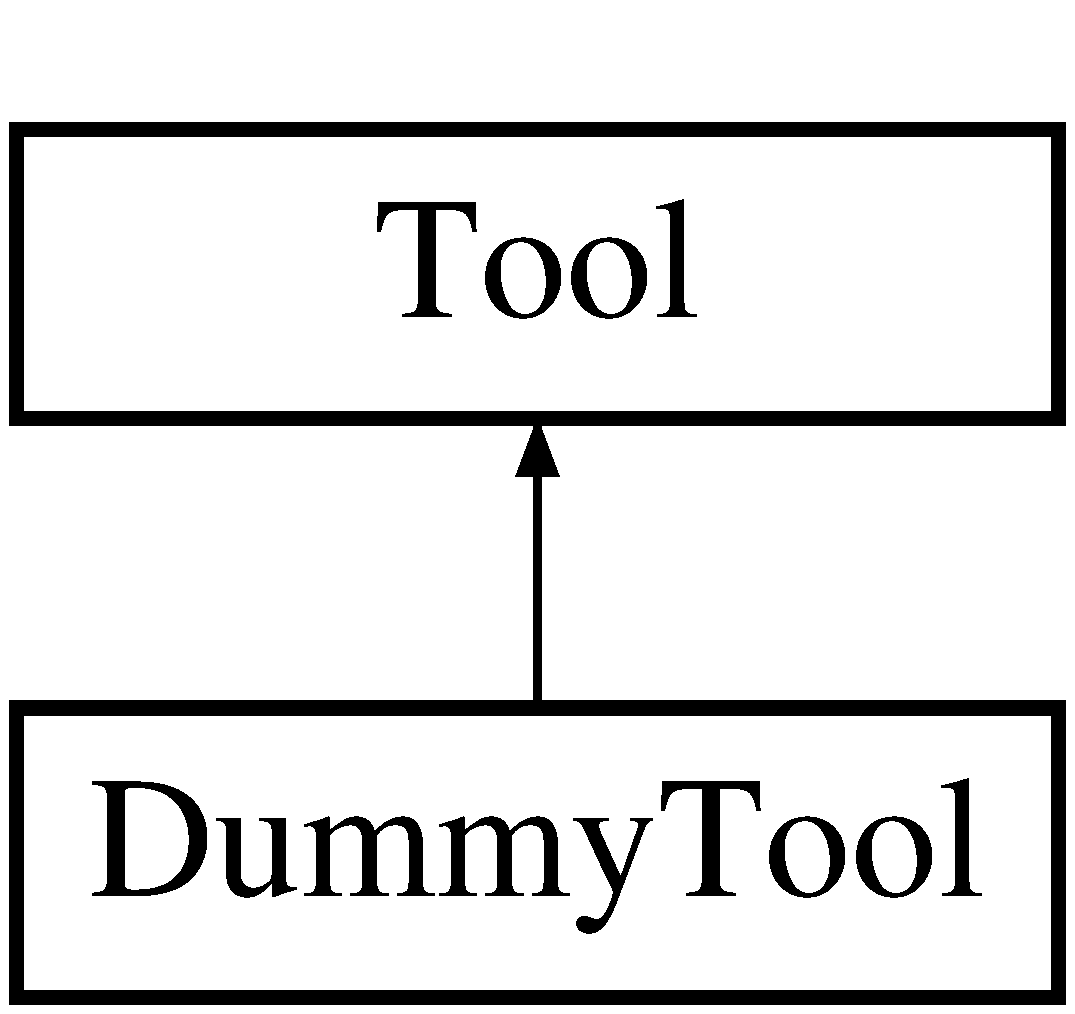
\includegraphics[height=2.000000cm]{classDummyTool}
\end{center}
\end{figure}
\subsection*{Public Member Functions}
\begin{DoxyCompactItemize}
\item 
\hypertarget{classDummyTool_a33914471b4de346168aa92b5febb6f9c}{\hyperlink{classDummyTool_a33914471b4de346168aa92b5febb6f9c}{Dummy\-Tool} ()}\label{classDummyTool_a33914471b4de346168aa92b5febb6f9c}

\begin{DoxyCompactList}\small\item\em Constructor. \end{DoxyCompactList}\item 
\hypertarget{classDummyTool_a0d9cd781681a06ee3cf0cd1e7bb770a8}{bool \hyperlink{classDummyTool_a0d9cd781681a06ee3cf0cd1e7bb770a8}{Initialise} (std\-::string configfile, \hyperlink{classDataModel}{Data\-Model} \&data)}\label{classDummyTool_a0d9cd781681a06ee3cf0cd1e7bb770a8}

\begin{DoxyCompactList}\small\item\em Assigns verbosity from config file and creates a log message. \end{DoxyCompactList}\item 
\hypertarget{classDummyTool_ac107b31f1785c1cc803e0e65be548047}{bool \hyperlink{classDummyTool_ac107b31f1785c1cc803e0e65be548047}{Execute} ()}\label{classDummyTool_ac107b31f1785c1cc803e0e65be548047}

\begin{DoxyCompactList}\small\item\em Creates a log message. \end{DoxyCompactList}\item 
\hypertarget{classDummyTool_aacb5d0b9906a27c2b4bba4aae9bc093a}{bool \hyperlink{classDummyTool_aacb5d0b9906a27c2b4bba4aae9bc093a}{Finalise} ()}\label{classDummyTool_aacb5d0b9906a27c2b4bba4aae9bc093a}

\begin{DoxyCompactList}\small\item\em Does nothing. \end{DoxyCompactList}\end{DoxyCompactItemize}


\subsection{Detailed Description}
This is a simple dummy Tool designed to show operation of a Tool. It also provides a default Tool for the Default Tool\-Chain.

\begin{DoxyParagraph}{Author\-:}
B.\-Richards 
\end{DoxyParagraph}
\begin{DoxyParagraph}{Date\-:}
2019/05/28 10\-:44\-:00 
\end{DoxyParagraph}
Contact\-: \href{mailto:b.richards@qmul.ac.uk}{\tt b.\-richards@qmul.\-ac.\-uk} 

The documentation for this class was generated from the following files\-:\begin{DoxyCompactItemize}
\item 
User\-Tools/\-Examples/Dummy\-Tool.\-h\item 
User\-Tools/\-Examples/Dummy\-Tool.\-cpp\end{DoxyCompactItemize}

\hypertarget{classMyTool}{
\section{MyTool Class Reference}
\label{classMyTool}\index{MyTool@{MyTool}}
}


{\ttfamily \#include $<$MyTool.h$>$}\subsection*{Public Member Functions}
\begin{DoxyCompactItemize}
\item 
\hypertarget{classMyTool_ad85b796bdd675ae22e69cf40fe7b6314}{
\hyperlink{classMyTool_ad85b796bdd675ae22e69cf40fe7b6314}{MyTool} ()}
\label{classMyTool_ad85b796bdd675ae22e69cf40fe7b6314}

\begin{DoxyCompactList}\small\item\em Simple constructor. \item\end{DoxyCompactList}\item 
bool \hyperlink{classMyTool_a3bf60061195a18542c4cfb2916b9dad9}{Initialise} (std::string configfile, \hyperlink{classDataModel}{DataModel} \&data)
\begin{DoxyCompactList}\small\item\em Initialise Function for setting up Tool resources. \item\end{DoxyCompactList}\item 
\hypertarget{classMyTool_a0a58122023af90b9200d0e71e89cfb36}{
bool \hyperlink{classMyTool_a0a58122023af90b9200d0e71e89cfb36}{Execute} ()}
\label{classMyTool_a0a58122023af90b9200d0e71e89cfb36}

\begin{DoxyCompactList}\small\item\em Execute function used to perform Tool purpose. \item\end{DoxyCompactList}\item 
\hypertarget{classMyTool_a060ec6356451aa335d0de41093c9992f}{
bool \hyperlink{classMyTool_a060ec6356451aa335d0de41093c9992f}{Finalise} ()}
\label{classMyTool_a060ec6356451aa335d0de41093c9992f}

\begin{DoxyCompactList}\small\item\em Finalise function used to clean up resources. \item\end{DoxyCompactList}\end{DoxyCompactItemize}


\subsection{Detailed Description}
This is a blank template for a Tool used by the script to generate a new custom tool. Please fill out the description and author information.

Author}
B.Richards Date}
2019/05/28 10:44:00 Contact: \href{mailto:b.richards@qmul.ac.uk}{\tt b.richards@qmul.ac.uk} 

\subsection{Member Function Documentation}
\hypertarget{classMyTool_a3bf60061195a18542c4cfb2916b9dad9}{
\index{MyTool@{MyTool}!Initialise@{Initialise}}
\index{Initialise@{Initialise}!MyTool@{MyTool}}
\subsubsection[{Initialise}]{\setlength{\rightskip}{0pt plus 5cm}bool MyTool::Initialise (std::string {\em configfile}, \/  {\bf DataModel} \& {\em data})}}
\label{classMyTool_a3bf60061195a18542c4cfb2916b9dad9}


Initialise Function for setting up Tool resources. 
\begin{DoxyParams}{Parameters}
\item[{\em configfile}]The path and name of the dynamic configuration file to read in. \item[{\em data}]A reference to the transient data class used to pass information between Tools. \end{DoxyParams}


The documentation for this class was generated from the following files:\begin{DoxyCompactItemize}
\item 
UserTools/template/MyTool.h\item 
UserTools/template/MyTool.cpp\end{DoxyCompactItemize}

%--- End generated contents ---

% Index
\newpage
\phantomsection
\addcontentsline{toc}{part}{Index}
\printindex

\end{document}
